\chapter{Progetto}
\label{chap:Progetto}

Nel presente capitolo, si analizza in dettaglio sia il contesto lavorativo che la realizzazione pratica del progetto che ha caratterizzato la mia esperienza di stage curriculare presso l'azienda Alten Italia. L’obiettivo è quello di fornire una visione dell’ambiente in cui ho vissuto l'esperienza di stage, nonché di presentare il progetto che ho avuto l'opportunità di realizzare.\\
Principalmente, si analizza in che modo il contesto lavorativo ha permesso la realizzazione e l'implementazione del progetto, che consiste nella creazione di un servizio back-end REST dedicato alla validazione degli ID bancari (IBAN), unitamente alla creazione di una pagina web SPA (\textit{Single Page Application}) per l'inserimento dei dati e la visualizzazione dei relativi output.\\
Innanzitutto, l'analisi si sofferma su una panoramica dell'azienda ospitante, fornendo una sintesi delle sue caratteristiche e delle sue attività principali. In secondo luogo, sono presentati gli obiettivi iniziali dello stage e le attività svolte, contestualizzando il progetto all'interno del quadro complessivo dell'esperienza. Viene poi descritto il progetto stesso, evidenziandone il ruolo all’interno dell’azienda e del panorama bancario attuale, al fine di comprendere come si integri in un contesto più ampio. Infine, viene analizzata nel dettaglio la realizzazione pratica del servizio web REST per la validazione di ID bancari e l’implementazione della corrispondente pagina web SPA, illustrando i particolari tecnici che ne sono alla base.

%%%%%%%%%%%%%%%%%%%%%%%%%%%%%%%%%%%%%%%%%%%%%%%%%%%%%%%%%%%%%%%%%%%%%%%%%%%%%%%%
\clearpage
\section{Contesto Lavorativo}

\subsection{ALTEN}

Alten è una società di consulenza specializzata in innovazione tecnologica e ingegneristica, fondata in Francia nel 1988.\\
Attualmente, il gruppo Alten, leader europeo nel campo della consulenza, rappresenta una multinazionale presente in più di 30 paesi in tutto il mondo. Questa vasta presenza globale la posiziona come azienda di riferimento in varie nazioni, riunendo una squadra che vanta oltre 54.000 dipendenti e collaboratori. Anche in Italia, Alten continua ad espandersi, operando su tutto il territorio nazionale e contando circa 4.000 dipendenti, con uffici distribuiti nelle principali città del Paese.\\
Alten si distingue nel mercato per la sua vasta gamma di servizi in ambito IT, ingegneristico e delle scienze della vita. Attraverso la progettazione e lo sviluppo di sistemi e interfacce utilizzando tecnologie all'avanguardia e durature nel tempo, Alten offre supporto e consulenza in diversi settori, tra cui servizi finanziari, industriali, automotive e molti altri. Inoltre, è impegnata nell’implementazione di progetti complessi e tecnologici lungo l’intera catena di sviluppo del prodotto per aziende leader in diversi settori. Parallelamente, Alten ha acquisito un ruolo chiave nei principali ambiti delle \textit{Life Sciences}, collaborando con vari CDMO (\textit{Contract Development and Manufacturing Organization}) di medie dimensioni e aziende farmaceutiche e biotecnologiche. Oltre a quanto presentato finora, l'azienda offre anche servizi di eccellenza, quali l’ingegneria per la ricerca e lo sviluppo, le strutture commerciali ed il supporto ai processi e alle tecnologie di produzione. L’obiettivo è garantire conformità, scalabilità e flessibilità lungo tutta la catena del valore.

\subsection{Stage e Obiettivi}
Gli obiettivi dell’esperienza di stage presso Alten Italia sono stati delineati con l’intento di massimizzare il valore formativo, sia dal punto di vista personale che aziendale. Prima dell’inizio dello stage, infatti, ho identificato alcuni principali obiettivi personali:
\begin{enumerate}
    \item \textbf{Apprendimento Tecnico Avanzato}, che mira ad approfondire le competenze pratiche nell’ambito dello sviluppo di servizi web e dell’implementazione di pagine web SPA, e ad acquisire una maggiore conoscenza nell’utilizzo di tecnologie e protocolli all’avanguardia.
    \item \textbf{Collaborazione Team-Oriented}: volevo migliorare le mie capacità di collaborazione all’interno di un team multidisciplinare e dislocato sul territorio. L’obiettivo era comprendere come le varie competenze tecniche si integrassero per raggiungere gli obiettivi aziendali.
    \item \textbf{Acquisizione di Responsabilità}: ho identificato l’assunzione delle responsabilità lavorative come uno degli obiettivi principali per essere in grado di analizzare e comprendere le situazioni di lavoro e per poter eseguire le mie mansioni nei tempi e nei modi previsti, migliorando le mie abilità di \textit{problem solving} e rispetto delle \textit{deadline}.
\end{enumerate}

Parallelamente, gli obiettivi aziendali sono stati allineati alle esigenze dell'azienda e al progetto che ho contribuito a sviluppare:
\begin{enumerate}
    \item \textbf{Formazione}: indirizzata all’apprendimento del framework di sviluppo proprietario del cliente, allo studio dei \textit{tool} necessari all’attività lavorativa e all’inserimento nel contesto lavorativo
    \item \textbf{Sviluppo del Servizio}: l’azienda aveva l’obiettivo di realizzare un servizio web REST affidabile e performante per la validazione degli ID bancari, con elevati standard di qualità e precisione. Al tempo stesso, l’azienda mirava a fornire un’interfaccia utente semplice ed intuitiva per accedere al servizio, offrendo un’esperienza d’uso gradevole e piacevole.
    \item \textbf{Integrazione Tecnologica}: per il progetto era cruciale adottare tecnologie all’avanguardia, che fossero moderne e scalabili, per garantire un’implementazione efficace e futura espandibilità.
\end{enumerate}

Attraverso la convergenza degli obiettivi personali e aziendali, l’esperienza di stage ha assunto una duplice natura: da un lato, ho avuto l’opportunità di apprendere e mettere in pratica competenze tecniche avanzate; dall’altro, ho contribuito al raggiungimento degli obiettivi aziendali, integrando con successo il mio progetto nel contesto lavorativo. Infatti, durante il periodo di stage, ho avuto l'opportunità unica di lavorare a stretto contatto con un team dedicato a un importante gruppo bancario europeo, con il compito principale di realizzare una \textit{web application} in grado di validare i codici IBAN, un elemento cruciale nel settore bancario.\\
Questo progetto è nato in risposta alle esigenze specifiche dell'azienda cliente, che aveva l'obiettivo di migliorare l'efficienza dei processi interni di verifica dei codici IBAN, rendendoli rapidi ed intuitivi. La mia sfida è stata quella di sviluppare una soluzione tecnologica robusta e precisa che potesse soddisfare i rigorosi standard del settore bancario europeo, creando un prodotto che fosse semplice nell’utilizzo e al tempo stesso affidabile.\\
La realizzazione della \textit{web application} ha richiesto la convergenza di competenze provenienti da diversi campi dello sviluppo software, dalla programmazione back-end alla progettazione front-end. L'approccio multidisciplinare è stato possibile grazie al contesto lavorativo di Alten, che promuove una cultura di collaborazione e apprendimento continuo.

\section{Architettura del Sistema e Interaction Diagram}

Come anticipato precedentemente, la realizzazione di un servizio semplice e affidabile per la validazione dei codici IBAN è stato l’obiettivo centrale del progetto. Prima di analizzare in dettaglio ogni sezione, è fondamentale delineare in maniera chiara la struttura e l’architettura complessiva dell’applicazione, esaminado parallelamente il caso d’uso principale.

\begin{figure}[H]
  \centering
  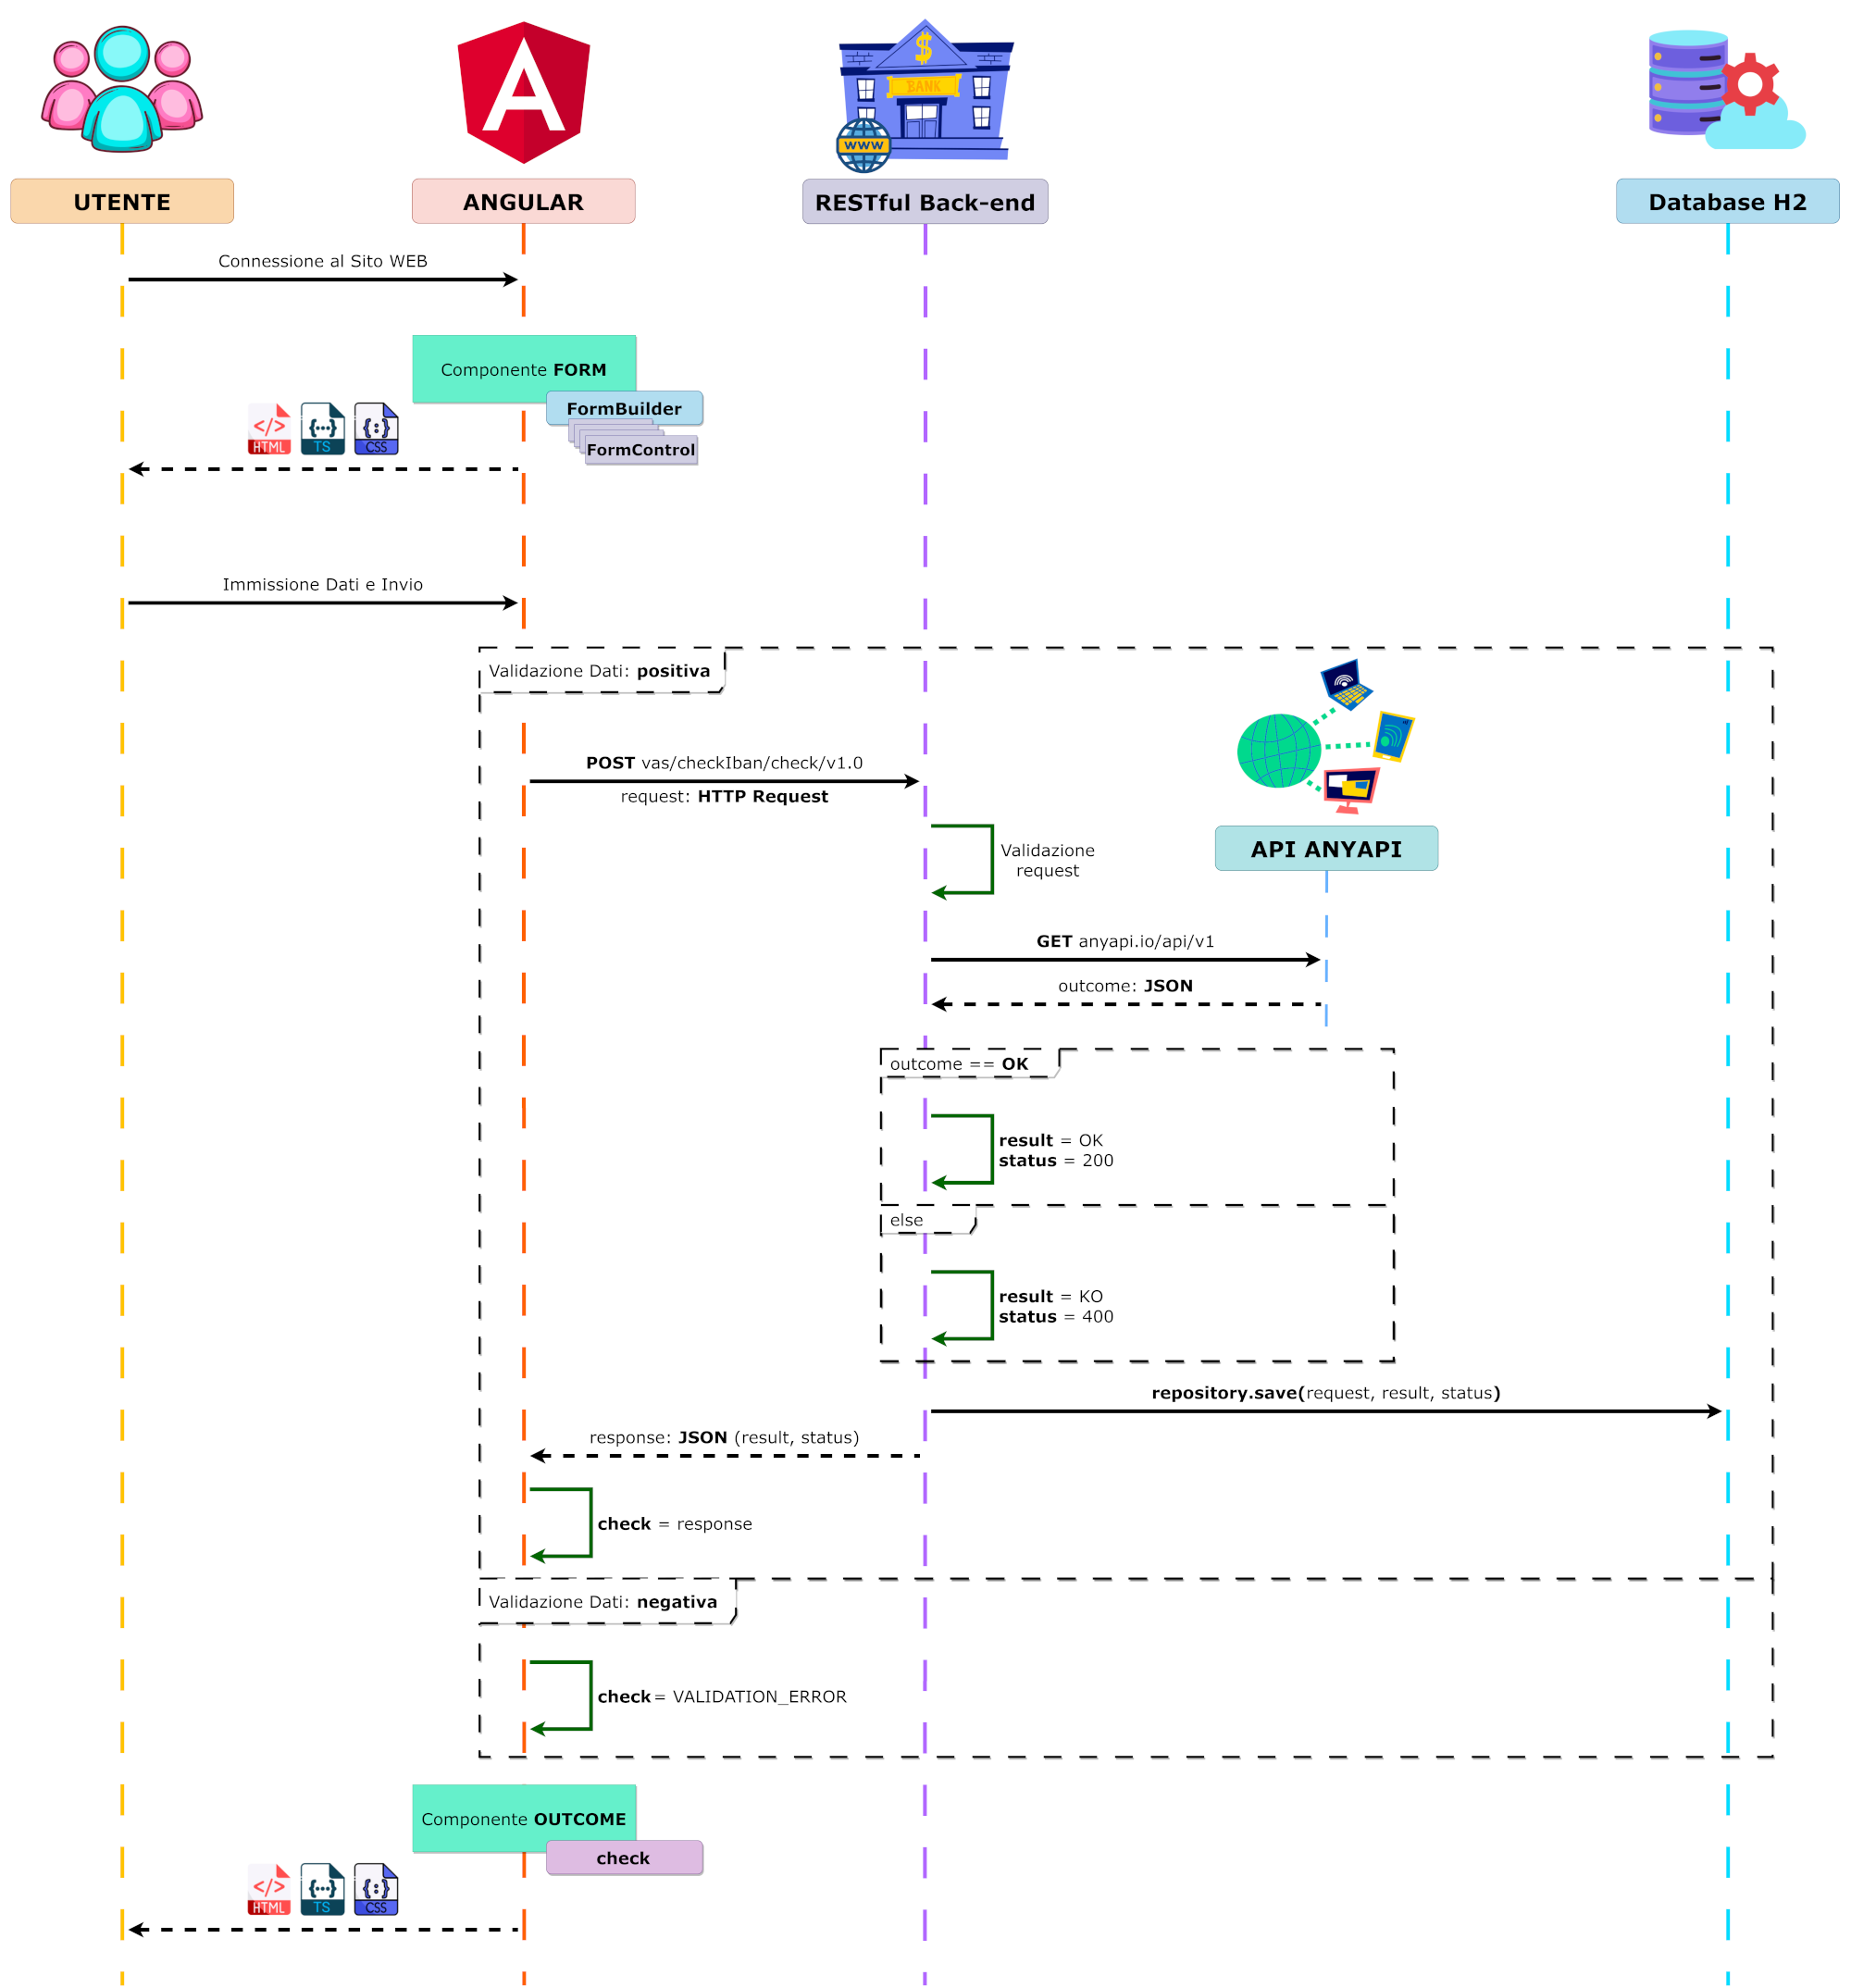
\includegraphics[width=1\textwidth]{img/Architettura.png}
  \caption{Caso d’uso principale del servizio, che comprende ogni componente realizzato e mostra le interazioni e il flusso logico dell’intera applicazione.} 
  \label{fig:Architettura.png}
\end{figure}
Il punto d’ingresso dell’applicazione è rappresentato da una \textit{web application} realizzata con il framework Angular. Il componente chiave esposto all’utente è un modulo di inserimento dati creato su misura, progettato per consentire l’inserimento accurato delle informazioni necessarie per effettuare la richiesta HTTP da inviare all’API REST fornita dal back-end. Questo modulo fornisce anche un primo livello di controllo sui dati inseriti, filtrando le informazioni per prevenire l’invio di richieste errate o dati in formati non supportati. Ciò minimizza la probabilità che il back-end interpreti erroneamente le richieste.\\
Proseguendo nell’architettura, la richiesta generata dal componente Angular viene ricevuta e processata dall’API RESTful esposta dal servizio back-end. Di seguito si illustrano i componenti e la struttura di questa sezione del progetto:
\begin{figure}[H]
  \centering
  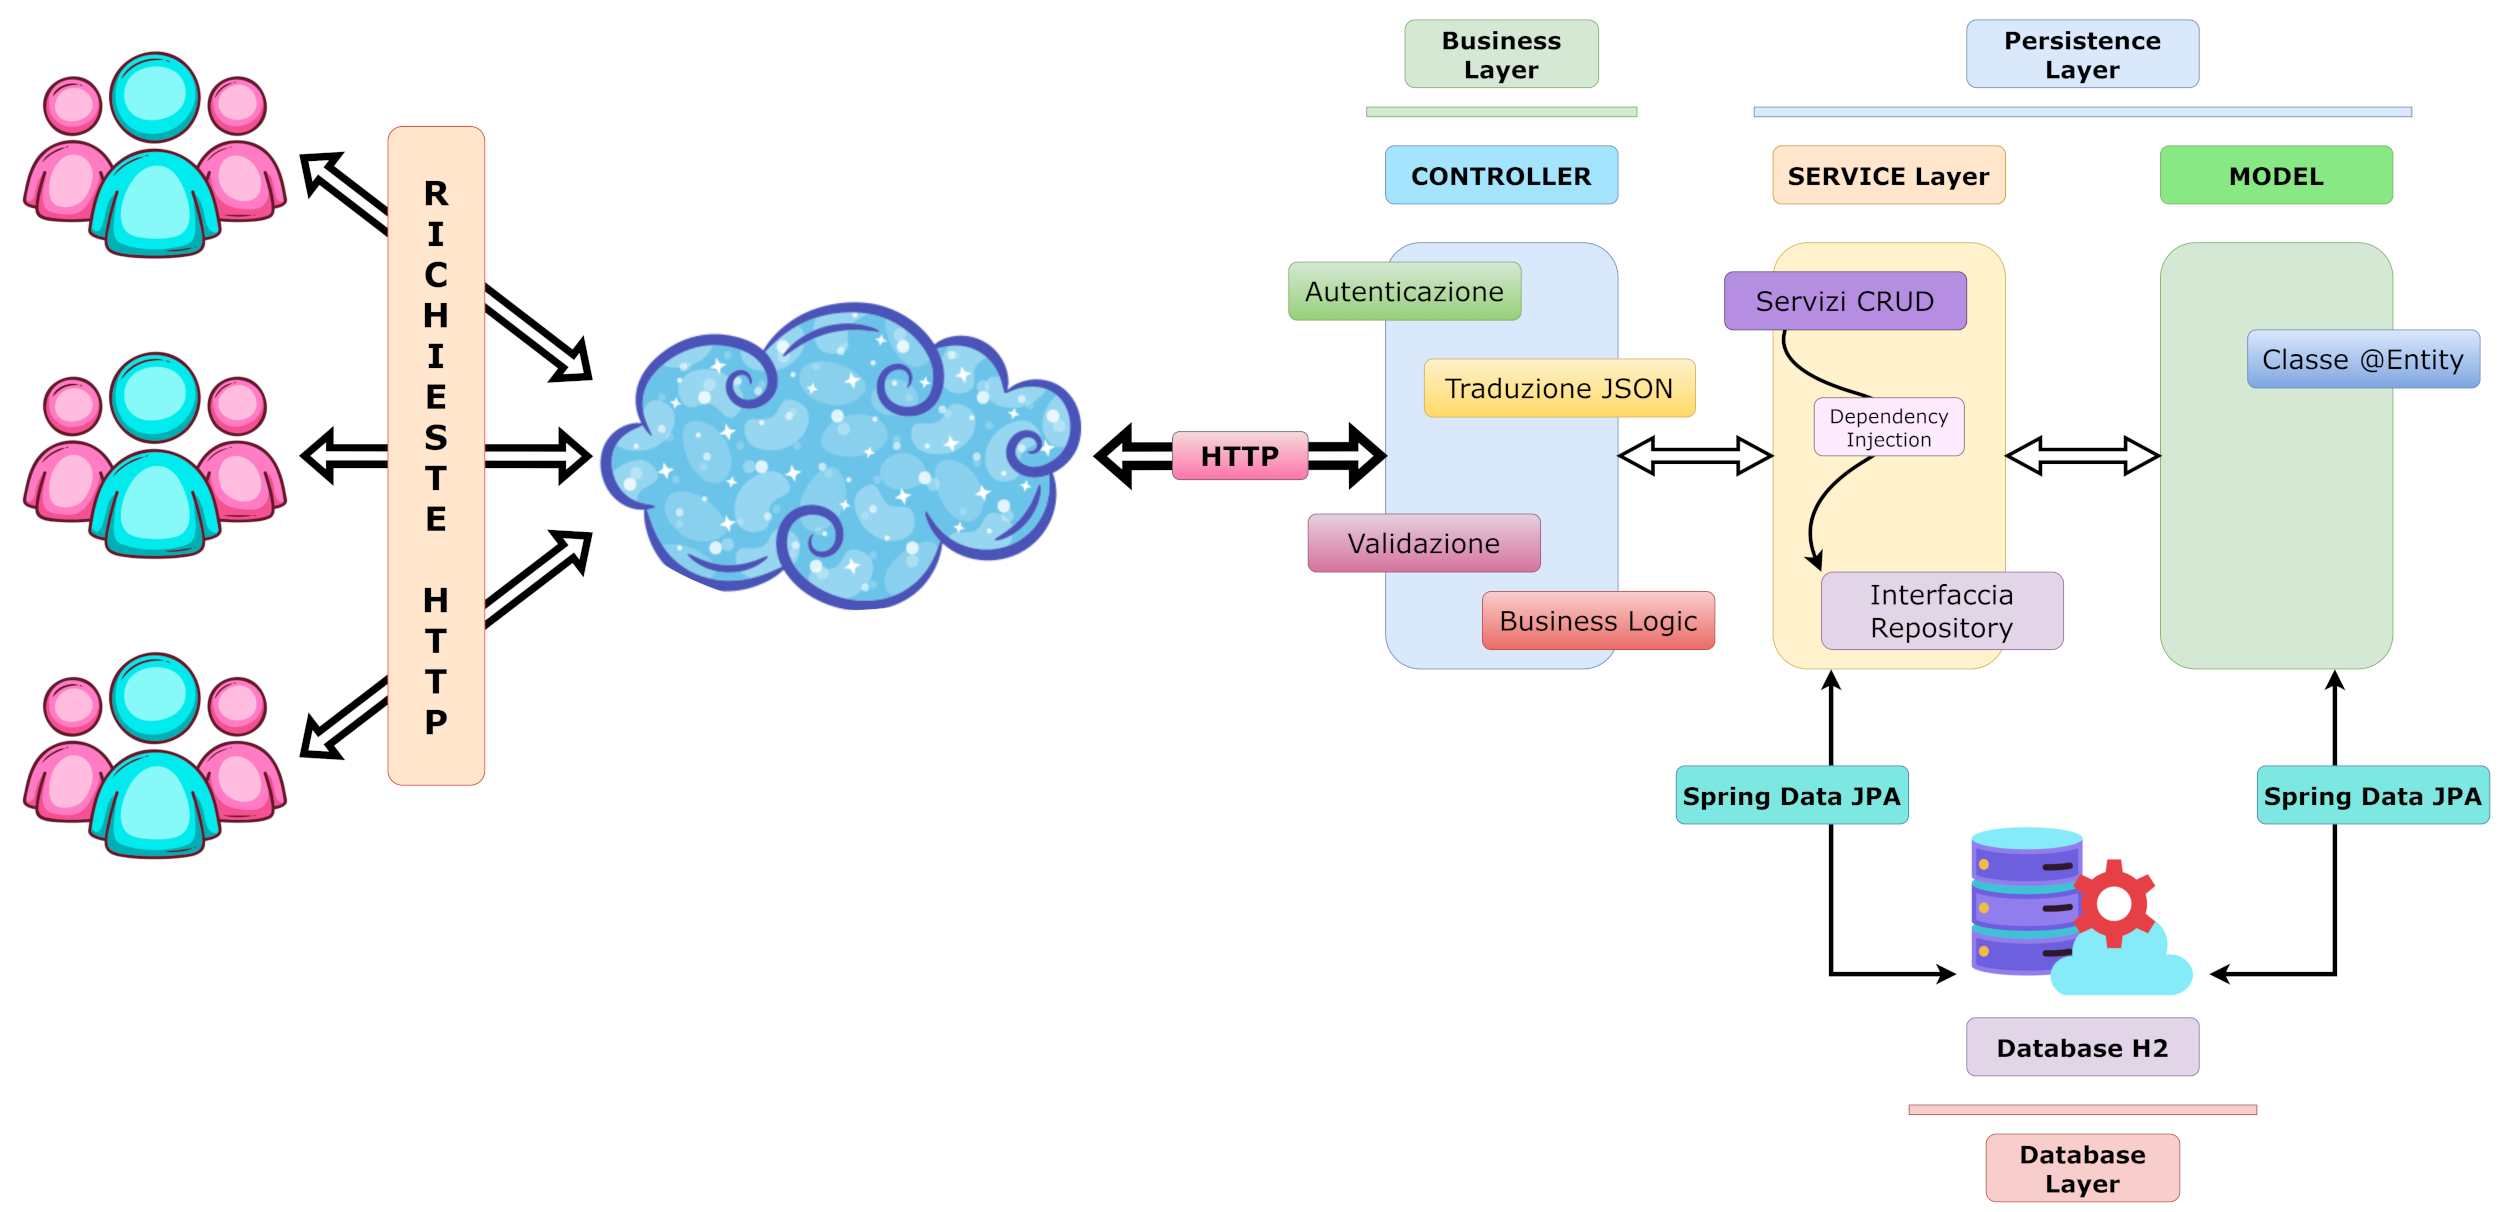
\includegraphics[width=1\textwidth]{img/SpringBoot_Diagramma.png}
  \caption{Rappresentazione dell’architettura back-end, illustrando la suddivisione logica del software e le interazioni.} 
  \label{fig:SpringBoot_Diagramma.png}
\end{figure}
Quando un \textit{client} invia una richiesta HTTP al servizio RESTful esposto dal back-end, questa viene ricevuta e gestita dal \textit{controller}, che agisce come livello di business. In questa circostanza, la richiesta viene scomposta in \textit{header} e \textit{body} e vengono prelevate le informazioni ricevute in formato JSON. Inoltre, il \textit{controller} è responsabile della gestione della logica di business dell’applicazione, come ad esempio l’elaborazione delle informazioni al fine offerto dal servizio, ovvero la validazione effettiva del codice IBAN.\\
Successivamente, avviene una transizione virtuale da livello di business a livello di persistenza, rappresentata con il passaggio dal \textit{controller} al \textit{service layer}. Questo componente logico opera sui dati mappati da Spring Data JPA con le classi del \textit{model} ed offre un’interfaccia \textit{Repository} per comunicare con il database. Oltre a ciò, il service layer consente l’applicazione della logica di archiviazione e la traduzione degli oggetti di business in righe del database e viceversa.\\
Il \textit{model}, già menzionato in precedenza, è composto dalle classi entità, che rappresentano gli oggetti Java corrispondenti alle righe del database.\\
\textit{Service layer} e \textit{model} collaborano sinergicamente per interagire con il livello di database, implementato con il DBMS H2. Sfruttando le logiche e i meccanismi messi a disposizione da Spring Data JPA, e rispettando le esigenze specifiche del database utilizzato, lo scambio di dati in entrata ed in uscita avviene in modo rapido e sicuro.\\
Infine, Spring Data fornisce annotazioni e interfacce appositamente create per agevolare l’implementazione della logica di archiviazione, consentendo agli sviluppatori di configurare rapidamente e in modo affidabile la struttura di comunicazione con il database.

\section{Back-end}

Lo sviluppo del progetto ha avuto come punto di inizio la realizzazione del servizio REST back-end, che costituisce il cuore del sistema di validazione degli IBAN. La realizzazione di questo componente, messa in pratica utilizzando il framework Spring Boot e, di conseguenza, il linguaggio di programmazione Java, ha richiesto un'attenta pianificazione, l'adozione delle migliori pratiche di sviluppo, e un'analisi dettagliata dei requisiti dell'azienda cliente.\\
Inoltre, per garantire l’integrità e la tracciabilità dei dati, è stato espressamente indicato nei requisiti di implementare un sistema di registrazione delle richieste su database H2 in-memory. Ciò ha richiesto l'utilizzo del framework Spring Data JPA per creare entità e \textit{repository} dedicati all'accesso al database, tali da garantire la persistenza delle informazioni relative alle richieste effettuate, consentendo una visione d'insieme e una possibile analisi dei dati raccolti.\\
Infine, è stato applicato il principio della testabilità tramite lo sviluppo di una suite di test automatizzati, grazie all’implementazione del \textit{tool} JUnit. Questi test hanno lo scopo di verificare la corretta funzionalità dei metodi sviluppati e di rilevare eventuali errori o \textit{bug} in modo preventivo.

\section{Servizio REST}

Come anticipato, il cuore dello sviluppo back-end dell’applicazione è l’esposizione del servizio REST basato su Spring Boot. Questo strato di servizio è responsabile per la gestione delle richieste HTTP provenienti dai \textit{client} e per la fornitura di risposte appropriate in modo efficiente e scalabile.\\
Innanzitutto, Spring Boot mette a disposizione una base solida dalla quale partire per realizzare un applicativo, generando un progetto basilare ma composto da tutte le dipendenze necessarie. Tra queste, per abilitare l'esposizione del servizio REST svolge un ruolo chiave il componente «\texttt{Spring Web}», che inoltra con precisione le richieste HTTP alle risorse dell'applicazione pertinenti e gestisce la generazione e il rilascio delle risposte ai \textit{client}, formattate come oggetti JSON. La sua integrazione abilita un flusso coerente delle richieste e delle risposte, garantendo un'esperienza utente ottimale.\\
Per quanto riguarda il processo di validazione delle richieste in arrivo, riveste una grande importanza la dipendenza «\texttt{Validation}». Questo strumento gioca un ruolo cruciale per garantire che i dati forniti dai \textit{client} rispettino le regole definite dal programmatore. In tal modo, si assicura che le richieste ricevute siano affidabili e adeguate all'elaborazione.\\
Un'altra componente vitale è «Spring Data JPA», impiegata per la persistenza dei dati relativi alle richieste. Questo componente si interfaccia direttamente con il database, consentendo la memorizzazione accurata delle informazioni sulle richieste effettuate dai \textit{client}. La possibilità di interagire con il database facilita la tracciabilità delle richieste, un requisito fondamentale per l'azienda cliente. La scelta di impiegare l'«H2 Database», un database in-memory, offre un vantaggio notevole in termini di velocità di esecuzione. Questo database, integrato nell'applicazione, garantisce un meccanismo di archiviazione efficiente e temporaneo per i dati, contribuendo così all'ottimizzazione complessiva del sistema.\\
Questi componenti collaborano per fornire un servizio affidabile e scalabile, gestendo le richieste, validando i dati in ingresso, consentendo la tracciabilità delle operazioni e garantendo un'archiviazione efficiente dei dati. L'integrazione di queste tecnologie contribuisce in modo significativo all'efficienza e alla robustezza del sistema. Inoltre, tutto questo è facilmente configurabile tramite uno strumento messo a disposizione da Spring, noto come Spring Initializr, usufruibile sia tramite l’omonimo sito web sia tramite l’estensione compatibile con tutti i principali IDE.
\begin{figure}[H]
  \centering
  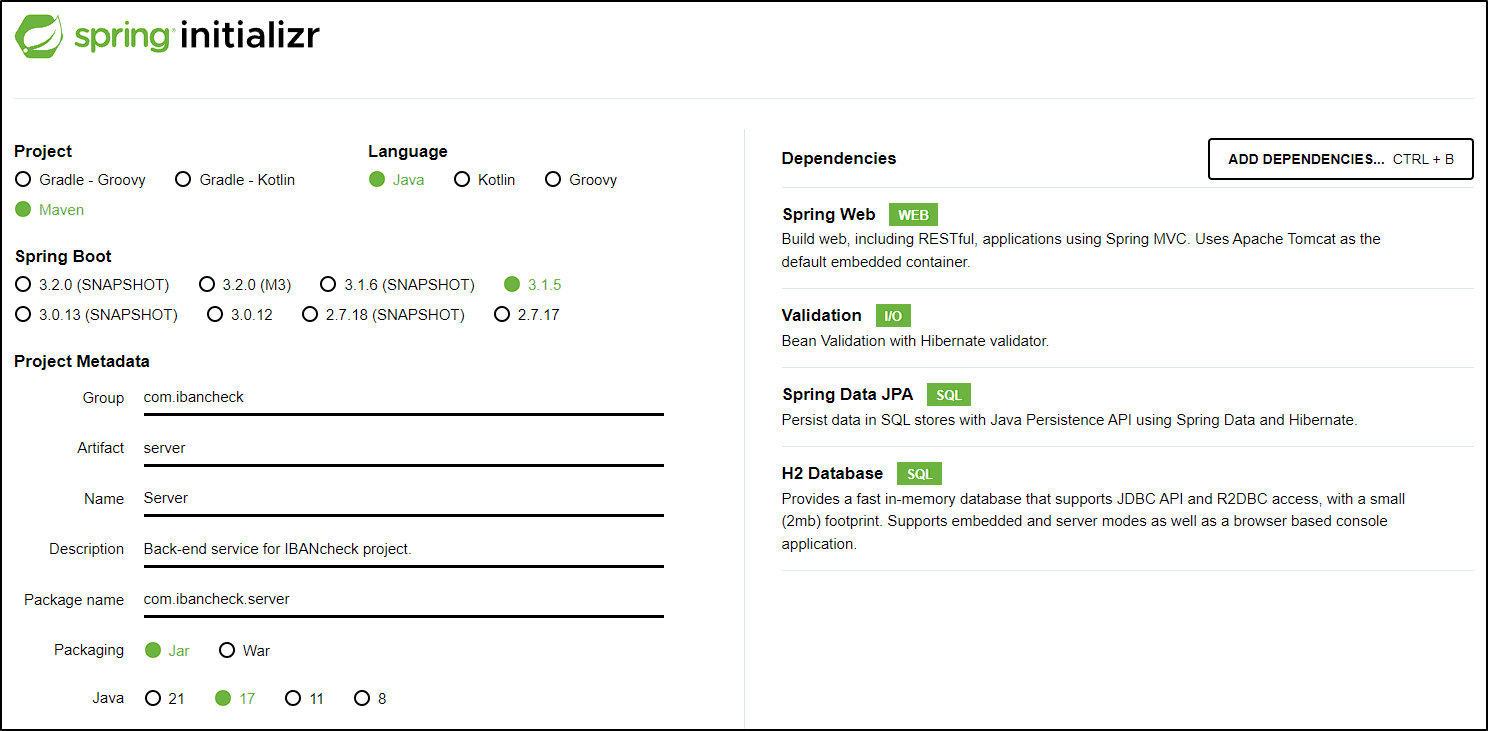
\includegraphics[width=0.9\textwidth]{img/Spring-Initializr.png}
  \caption{Configurazione iniziale del progetto e selezione delle dipendenze via Spring Initializr, da sito web.} 
  \label{fig:Spring-Initializr.png}
\end{figure}
Infine, la configurazione del programma è gestita principalmente attraverso il file \textit{pom.xml}, in cui vengono definite le dipendenze e le versioni dei linguaggi e framework usati.

\section{Controller}
Una volta scaricato il progetto configurato con Spring Initializr, è possibile aprirlo in un IDE a piacere per personalizzarne il codice sorgente e aggiungere tutte le funzionalità necessarie. Nel contesto di un servizio web REST sviluppato con Spring Boot, si semplifica l'uso del \textit{design pattern Model-View-Controller} (MVC). In questo modo, il \textit{Model} rappresenta i dati e le risorse, il \textit{Controller} coordina le richieste, mentre la \textit{View} è sostituita dalla rappresentazione dei dati inviati ai \textit{client}, tipicamente in formato JSON. Tale organizzazione offre una struttura chiara per gestire le richieste e le risposte nei servizi RESTful.\\
Per iniziare, è necessario creare una classe Java che funga da \textit{controller} e annotarla con \texttt{@RestController}, che semplifica la creazione di servizi web RESTful. Questa annotazione rappresenta una versione specializzata del \textit{controller}, combinando le funzionalità offerte da \texttt{@Controller} e \texttt{@ResponseBody}.\\
Inoltre, si aggiunge l’annotazione \texttt{@RequestMapping} per definire il percorso di base per accedere ai vari metodi esposti dalla classe. Nonostante il caso specifico preveda un \textit{controller} con attualmente un solo metodo accessibile dall'esterno, questa impostazione diventa utile se si prevede di implementare ulteriori metodi in futuro. Quindi, per il momento, si definisce il \textit{mapping} della richiesta sul percorso \texttt{vas/checkIban/check}, lasciando al singolo metodo la possibilità di specificare solo la versione del servizio:
\begin{lstlisting}[language=Java, caption=Implementazione della classe controller.]
@RestController
@RequestMapping("vas/checkIban/check")
public class ApplicationCheckController \{
		//Codice della classe...
}
\end{lstlisting}
La cosa principale da notare, per quanto mostrato finora, è l’assenza della necessità di importare manualmente le librerie nel \textit{workspace} per utilizzarle. Infatti, vengono dichiarate nel file \textit{pom.xml} in modo che Maven possa risolverle automaticamente, scaricarle ed utilizzarle per la compilazione dell’eseguibile in formato JAR.\\
Successivamente, si prosegue con la creazione del metodo principe della classe\\
\texttt{ApplicationCheckController}. Questo è responsabile di gestire le richieste di tipo POST, ricevute tramite il protocollo HTTP, che forniscono parametri sia nell’\textit{header} che nel \textit{body}.

\subsubsection{Validazione dei Dati}

Prima di poter proseguire con la validazione del codice IBAN inviato nella richiesta, è necessario verificare la correttezza dei dati forniti al servizio. Questo controllo viene effettuato in due modalità distinte, a seconda che le informazioni siano contenute nell’\textit{header} o nel \textit{body} della richiesta. Inoltre, è possibile definire il messaggio da restituire nel caso in cui il vincolo non sia soddisfatto.

\subsubsection{Parametri nell’Header}

Il caso più semplice riguarda i parametri nell’\textit{header}. È necessario specificare le proprietà che devono essere soddisfatte direttamente nella firma del metodo. Nel caso in questione, l’azienda cliente richiede di ricevere due stringhe non vuote: la prima con una lunghezza massima di 255 caratteri e la seconda di 20. La firma del metodo è quindi definita per rispettare tali requisiti:
\begin{lstlisting}[language=Java, caption=Dichiarazione dei parametri all'interno della firma del metodo.]
@RequestHeader(value = "x-request-id", required = true)
@Size(max = 255, message = "Request ID size out of range [max size = 255]") String requestId,
@RequestHeader(value = "subscriber-code", required = true)
@Size(max = 20, message = "Subscriber Code size out of range [max size = 20]") String subscriberCode
\end{lstlisting}
In questo caso, \texttt{@RequestHeader} specifica il nome del parametro presente nell’\textit{header} e fornisce l’attributo \texttt{required}. Quando impostato come nel caso attuale a \texttt{true}, rende valide solo le richieste contenenti quel parametro, escludendo stringhe vuote o nulle. Invece, l’annotazione \texttt{@Size} definisce la lunghezza delle stringhe. Nel caso in questione, è stato specificato solo l’attributo \texttt{max}, che rappresenta la lunghezza massima. Questo perché il controllo sul fatto che abbiano almeno 1 carattere è implicito nell’attributo \texttt{required} di \texttt{@RequestHeader}. Se fosse necessario avere una dimensione minima di \textit{n} caratteri, dove \textit{\texttt{n > 1}}, allora andrebbe specificato l’attributo \texttt{min} di \texttt{@Size}.

\subsubsection{Parametri nel Body}
Per quanto riguarda il \textit{body} della richiesta, la dinamica cambia leggermente. Tanto per cominciare, il tipo deve corrispondere a \texttt{JSON}, che è necessario per effettuare il \textit{parsing} in un oggetto Java, così da accedere ai dati contenuti. Questo viene realizzato attraverso la creazione di un oggetto \texttt{Provider} che riflette la struttura del JSON, seguito dall’impostazione dei vincoli di validità sugli attributi.
\begin{lstlisting}[language=Java, caption=Dichiarazione dei vincoli di validità per i dati contenuti nel \textit{body} della richiesta.]
@NotNull(message = "Provider Code cannot be null")
@Size(max = 20, message = "Provider Code size out of range [max size = 20]")
private String providerCode;
@NotNull(message = "Account ID cannot be null")
@Size(max = 34, message = "Account ID size out of range [max size = 34]")
@Pattern(regexp = "[A-Z]{2}[0-9]{2}[A-Z0-9]{1,30}|[A-Z0-9]{1,30}", message = "Account ID has invalid format")
private String accountId;
@Size(max = 16, message = "Tax Code size out of range [max size = 16]")
@Pattern(regexp = "([0-9a-zA-Z-+/]){0,16}", message = "Tax Code has invalid format")
private String taxCode;
@Size(max = 14, message = "Vat Code size out of range [max size = 14]")
@Pattern(regexp = "([0-9a-zA-Z]){0,14}", message = "Vat Code has invalid format")
private String vatCode;
\end{lstlisting}
In questo contesto, le informazioni obbligatorie consistono in \texttt{providerCode} e \texttt{accountId}, che sono gli unici attributi annotati con il vincolo \texttt{@NotNull}. Gli altri due attributi sono opzionali e, pertanto, non sono stati sottoposti alla stessa annotazione. Alcuni attributi presentano inoltre l’annotazione \texttt{@Pattern}, che specifica il \textit{pattern} che devono rispettare per poter essere considerati validi, basandosi su espressioni regolari.Il tag \texttt{@Size} opera in modo analogo a quanto visto per gli attributi nell’\textit{header}.\\
Una volta fatto ciò, il processo non è ancora concluso. All’interno del metodo del \textit{controller} in cui viene ricevuta la richiesta, è fondamentale indicare che il JSON deve essere convertito in un oggetto \texttt{Provider} e che i suoi attributi devono essere validati. Quindi, si dichiara il parametro nel metodo come \texttt{@Valid @RequestBody Provider}, affinché Spring identifichi quell’oggetto come la rappresentazione del JSON nel \textit{body} e ne effettui la validazione in base alle regole interne. Infine, per specificare il consumo di un JSON, il metodo è annotato con \texttt{@PostMapping(path = "/v1.0", consumes = "application/json", produces = "application/json")}. Ciò indica il percorso (\texttt{path}) specifico del metodo, il tipo di input proveniente dal \textit{body} ed il tipo di risposta restituito.

\subsection{Comunicazione con API Esterna}

Una volta validati tutti i dati necessari al servizio, si procede con il controllo del codice IBAN inserito per verificarne la correttezza. Tale procedura si basa sull’uso di un’API esterna fornita da \href{http://anyapi.io/}{anyapi.io}, con cui si stabilisce comunicazione direttamente dal \textit{controller}.

\subsubsection{Creazione del Data Transfer Object}

Per iniziare questa fase, si crea il \textit{Data Transfer Object} (DTO), un oggetto Java usato per lo scambio di dati, impiegato per mappare la risposta ottenuta dall’API esterna. A tal fine, è fondamentale comprendere la struttura della risposta fornita dal servizio \textit{anyapi}. In particolare, si tratta di un JSON del seguente formato:
\begin{lstlisting}[caption=Struttura del JSON restituito dall'API esterna.]
{   "valid": true,
    "iban": "BE68 5390 0754 7034",
    "countryCode": "BE",
    "bban": "539007547034",
    "electronicFormat": "BE68539007547034"   }
\end{lstlisting}
Ora che si conosce la struttura della risposta, bisogna creare una classe con attributi corrispondenti ai campi del JSON. Affinché la mappatura possa avvenire correttamente, è essenziale fornire i metodi \textit{getter} e \textit{setter} per ogni attributo. Inoltre, la classe deve implementare l’interfaccia \texttt{Serializable}; altrimenti, non potrebbe essere utilizzata negli scambi HTTP, e dunque non sarebbe di fatto un \textit{Data Transfer Object}. La classe risultante è la seguente:
\begin{lstlisting}[language=Java, caption=Classe \textit{Data Transfer Object} utilizzata per mappare la risposta dell'API esterna.]
public class Iban implements Serializable {
    private String iban;
    private boolean valid;
    private String countryCode;
    private String bban;
    private String electronicFormat;

    public Iban() {
    }
	// getter e setter...
}
\end{lstlisting}

\subsubsection{Utilizzo delle Informazioni da application.properties}

Al fine di migliorare la leggibilità e la coesione del codice, oltre ad agevolare l’individuazione delle variabili che contengono il \textit{link} e la chiave dell’API esterna, è stato scelto di collocare questi valori all’interno del file di configurazione \textit{application.properties}. A tal proposito, sono state create due variabili:
\begin{lstlisting}[caption=Dichiarazione delle variabili all'interno del file di configurazione.]
anyapi.api_key = ---chiave-api---
anyapi.url_template = https://anyapi.io/api/v1/iban?iban=%s&apiKey=%s
\end{lstlisting}
Nel codice, il \textit{controller} è annotato con \texttt{@PropertySource(value = \\"classpath:application.properties")}, specificando così il file di configurazione in cui effettuare la ricerca. Successivamente, vengono definite due variabili interne di tipo stringa:
\begin{itemize}
    \item \texttt{API\_KEY}
    \item \texttt{URL\_TEMPLATE}
\end{itemize}
Inoltre, è presente una variabile d’ambiente denominata \texttt{env}, di tipo \\\texttt{org.springframework.core.env.Environment}. Questa variabile è annotata con \\\texttt{@Autowired} e dev’essere privata, permettendo a Spring di iniettare automaticamente le dipendenze cercando un \textit{bean} gestito dal \textit{container} che corrisponda a quel tipo di dato (\texttt{Environment}), assegnandolo all’attributo. Infine, si utilizza il metodo \texttt{getProperty} di \texttt{env} per accedere al file di configurazione e recuperare il valore corrispondente, specificando il nome della variabile contenuta in \textit{application.properties}:
\begin{lstlisting}[language=Java, caption=Recupero delle informazioni per effettuare la chiamata all'API.]
API_KEY = env.getProperty("anyapi.api_key");
URL_TEMPLATE = env.getProperty("anyapi.url_template");
\end{lstlisting}

\subsubsection{Richiesta verso API Esterna}

Per avviare il processo di richiesta, una fase chiave coinvolge l'importazione della classe \texttt{org.springframework.web.client.RestTemplate}, che svolge un ruolo fondamentale nella comunicazione con le API esterne permettendo di effettuare richieste HTTP sincrone. Una volta dichiarata e istanziata una variabile di tipo \texttt{RestTemplate}, è possibile utilizzare il metodo \texttt{getForObject(String url, Class responseType)} per iniziare una richiesta HTTP di tipo \texttt{GET} all'URL specificato.\\
Questo metodo richiede due parametri principali:
\begin{enumerate}
    \item \textbf{\texttt{url}}: è l’indirizzo di destinazione, composto tenendo conto delle informazioni raccolte nella sezione antecedente.
    \item \textbf{\texttt{responseType}}: rappresenta la classe Java in cui si desidera convertire la risposta HTTP ricevuta dall'API esterna e corrisponde al \textit{Data Transfer Object} realizzato in precedenza.
\end{enumerate}
Si sottolinea che in caso di errore durante la richiesta, il metodo \texttt{getForObject} restituisce un valore \texttt{null}. Pertanto, è fondamentale eseguire un controllo immediatamente dopo la chiamata per verificare se l'oggetto risultante è stato popolato correttamente. Questa verifica è necessaria per confermare che la richiesta sia stata completata con successo. Nel caso in cui l'oggetto sia nullo, è fondamentale gestire l'errore in modo adeguato, stabilendo procedure di gestione degli errori in grado di garantire un comportamento affidabile da parte del sistema.

\section{Database}

Uno degli obiettivi principali del progetto è il tracciamento delle richieste al servizio di validazione dei codici IBAN. A tale scopo, è stato adottato un approccio che dà priorità alla velocità di esecuzione a discapito della memoria utilizzabile. Ciò è motivato dalla previsione iniziale di un basso numero di richieste. Pertanto, è stata scelta l’opzione di utilizzare un database in-memory conosciuto come H2.

\subsection{Schema SQL}
Anche in questa circostanza, il framework Spring, specialmente Spring Data, si rivela estremamente utile ed affidabile. Una volta integrate le dipendenze nel file \textit{pom.xml}, che grazie a Maven permette di scaricare ed utilizzare le librerie all’interno del progetto, è sufficiente definire un file SQL con lo scheletro della tabella da realizzare. Automaticamente , Spring implementa il database H2 secondo lo schema:
\begin{lstlisting}[language=SQL, caption=Schema SQL per la tracciatura delle richieste.]
DROP TABLE VALIDATION_LOGS IF EXISTS;
CREATE TABLE VALIDATION_LOGS (
    request_id VARCHAR(255) PRIMARY KEY,
    subscriber_code VARCHAR(20) NOT NULL,
    provider_code VARCHAR(20),
    response_code BIGINT NOT NULL,
    outcome VARCHAR(255) NOT NULL,
    error VARCHAR(255),
    iban_validated VARCHAR(255) NOT NULL,
    request_timestamp TIMESTAMP NOT NULL,
    response_timestamp TIMESTAMP NOT NULL
)
\end{lstlisting}
In questo caso, è importante precisare che, qualora non venga specificato un file SQL contenente lo schema per il database, Spring è in grado di crearne uno basandosi sulla classe (o eventuali più classi) annotata con \texttt{@Entity}.

\subsection{Entità}
Affinché Spring Data JPA possa mappare una classe ad una tabella del database, è necessario annotarla come entità. Inoltre, questa classe, chiamata in gergo tecnico POJO, deve avere un costruttore privo di argomenti ed un attributo che rappresenta la chiave primaria nella relativa tabella. A tale scopo, è stata implementata una classe chiamata \texttt{Persistence}, che funge da entità, in cui l’attributo \texttt{requestId} rappresenta la chiave primaria:
\begin{lstlisting}[language=Java, caption=Implementazione della classe entità.]
@Entity
@Table(name = "VALIDATION_LOGS")
public class Persistence {
    @Id
    @Column(name = "request_id", length = 255)
    private String requestId;
    @Column(name = "subscriber_code", nullable = false, length = 20)
    private String subscriberCode;
    @Column(name = "provider_code", nullable = true, length = 20)
    private String providerCode;
    @Column(name = "response_code", nullable = false, length = 3)
    private int responseCode;
    @Column(name = "error", nullable = true, length = 21)
    private String error;
    @Column(name = "outcome", nullable = false, length = 2)
    private String outcome;
    @Column(name = "iban_validated", nullable = false, length = 255)
    private String ibanValidated;
    @Column(name = "request_timestamp", nullable = false)
    @Temporal(TemporalType.TIMESTAMP)
    private Date requestTimestamp;
    @Column(name = "response_timestamp", nullable = false)
    @Temporal(TemporalType.TIMESTAMP)
    private Date responseTimestamp;

    public Persistence() {
    }
		// codice di getter e setter...
}
\end{lstlisting}
Esaminando l’implementazione dell’entità, emergono alcune particolarità:
\begin{itemize}
    \item Oltre ad essere annotata con \texttt{@Entity}, la classe è stata decorata con \texttt{@Table}. Questo per specificare il nome della tabella nel database che deve corrispondere all’entità, poiché nello schema SQL precedentemente esaminato abbiamo assegnato un nome diverso alla tabella rispetto a quello della classe entità.
    \item La chiave primaria della classe è annotata con \texttt{@Id}.
    \item Ogni attributo è annotato con \texttt{@Column}, che definisce il nome della colonna a cui corrisponde quell’attributo. In alcuni casi, definisce anche la lunghezza massima che può assumere un attributo e se può essere \texttt{null} oppure no. Questo consente una validazione preventiva prima che un oggetto venga salvato nel database, facilitando la rilevazione di errori prima della persistenza effettiva.
    \item I due attributi di tipo \texttt{Date} sono annotati con \texttt{@Temporal} per specificare il tipo di valore temporale a cui corrispondono. Naturalmente, questi valori devono coincidere con quelli definiti nello schema SQL.
\end{itemize}

\subsection{Repository}

Giunti a questo punto, sono disponibili tutti gli elementi necessari per stabilire un collegamento tra la tabella del database e l’entità Java. Vediamo come rendere effettiva questa comunicazione.\\
Spring Data JPA si concentra sull'utilizzo di JPA per salvare dati in database relazionali. La sua funzionalità più principale in quest’ambito è la capacità di creare automaticamente implementazioni di \textit{repository}, a runtime, partendo dalla definizione di un'interfaccia, chiamata appunto \textit{repository}. Quindi, è necessario creare un’interfaccia denominata \texttt{PersistenceRepository}, in grado di operare con entità \texttt{Persistence}:
\begin{lstlisting}[language=Java, caption=Implementazione dell'interfaccia Repository.]
public interface PersistenceRepository extends CrudRepository<Persistence, String> {
    Persistence findByRequestId(String requestId);
    List<Persistence> findBySubscriberCode(String subscriberCode);
    List<Persistence> findByProviderCode(String providerCode);
}
\end{lstlisting}
Innanzitutto, si osserva l’estensione di un’altra interfaccia, \texttt{CrudRepository}, che consente di specificare (attraverso i due parametri generici) il tipo dell’entità con cui operare ed il tipo di identificatore da utilizzare. Come specificato precedentemente, non è necessario definire una classe che implementi \texttt{PersistenceRepository} per usare i metodi qui definiti: Spring Data JPA si occupa di tutto in modo autonomo. Pertanto, è possibile definire tutti i metodi desiderati all’interno di questa interfaccia, per recuperare dati o persistere informazioni nel database. Successivamente, il framework farà assunzioni sulla firma dei metodi per garantire il corretto funzionamento di ciascuno.\\
Una volta completati questi passaggi, è possibile richiamare uno qualsiasi dei metodi definiti in \texttt{PersistenceRepository} o nell’interfaccia estesa \texttt{CrudRepository} per comunicare col database. Nel \textit{controller} dell’applicazione, quando arriva una nuova richiesta, la prima azione è verificare che l’\texttt{id} non sia già presente nel database. In caso affermativo, viene restituito immediatamente un errore. Per fare ciò, viene richiamato il metodo \texttt{findByRequestId(requestId)}.

\section{Front-end}

Il front-end dell’applicazione si basa interamente sul framework di sviluppo Angular, utilizzato per creare l’interfaccia utente dell’applicazione come \textit{Single Page Application}. La \textit{web application} è stata realizzata focalizzandosi sulla creazione e la comunicazione dei componenti, resa possibile da fondamentali script TypeScript, utilizzati anche per la presentazione dell’output nella pagina.

\section{Angular Web-Application}
L’architettura software di una \textit{web application} Angular è cruciale per garantire una struttura ben organizzata e scalabile del progetto. Infatti, una delle caratteristiche principali di questo framework è la modularità, che favorisce la suddivisione dell’applicativo e la comunicazione tra i vari componenti seguendo il \textit{pattern} architetturale MVC. Inoltre, Angular offre una vasta gamma di librerie e pacchetti che agevolano l’interazione con i servizi back-end, consentendo all’applicazione di recuperare le informazioni necessarie in tempo reale e di gestire le operazioni in modo sicuro.\\
Per iniziare a sviluppare un'applicazione Angular, è essenziale possedere anche Node.js e NPM. Senza entrare troppo nei dettagli, il primo offre un ambiente di esecuzione per il codice JavaScript, mentre il secondo è un registro di software \textit{open-source} per la gestione dei pacchetti. Nel caso in esame, NPM serve per recuperare il \textit{package} Angular CLI, che consente di creare un \textit{workspace} Angular con il comando \texttt{ng new <nome\_progetto>}, dove il nome del progetto corrisponde a \texttt{iban-check}.

\section{Componenti}

Nel contesto Angular, con il termine «componenti» si fa riferimento ai blocchi che compongono un’applicazione. Ogni componente è costituito da una classe TypeScript decorata con \texttt{@Component()}, un template HTML e degli stili CSS che definiscono l’aspetto degli elementi del template. Questi componenti possono essere creati utilizzando il comando \texttt{ng generate component <nome\_componente>} tramite Angular CLI.
Nel caso in esame, la \textit{web application} è formata da 4 componenti:
\begin{enumerate}
    \item \textbf{form} → rappresenta il modulo per l’inserimento dei dati;
    \item \textbf{offline} → costituisce la schermata da visualizzare se il servizio back-end non è raggiungibile;
    \item \textbf{outcome} → mostra il risultato dell’elaborazione del back-end;
    \item \textbf{top-bar} → è la barra superiore, presente in ogni schermata dell’applicazione.
\end{enumerate}
I componenti Angular sono il cuore dell'applicazione. Ognuno di essi è responsabile di un aspetto specifico dell'interfaccia utente e della logica di presentazione dei dati. Come esposto in precedenza, l'architettura software promuove la separazione dei compiti e la riutilizzabilità del codice attraverso la modularità. La comunicazione tra i componenti avviene tramite i servizi Angular e l'emissione di eventi personalizzati. Questa struttura permette di mantenere il codice più manutenibile e facilita lo sviluppo di front-end caratterizzati da un’interazione con l’utente complessa.

\subsection{Form di Immissione}

La pagina principale dell’applicazione, nonché il punto in cui l’utente inserisce i propri dati nel sistema, è rappresentata dal componente \texttt{form}. Come ogni componente, possiede un template HTML ed un file TypeScript, che contiene la logica e la definizione dei campi.
L’elemento \texttt{<form>} nel file HTML è legato ad un \texttt{FormGroup} presente nello script, in modo da effettuare direttamente la validazione dei campi:
\begin{lstlisting}[language=HTML, caption=\textit{Binding} dell'elemento \texttt{form} tra HTML e TypeScript.]
<form [formGroup]="ibanCheckForm">
\end{lstlisting}
All’interno del file TypeScript, il \texttt{FormGroup} è associato ad un \texttt{FormBuilder} ed ogni campo è rappresentato da un oggetto \texttt{FormControl}. In questo modo, è possibile implementare la validazione e definire il controllo automatico dei valori, così che l’applicazione eviti di effettuare richieste contenenti dati sintatticamente errati.
\begin{lstlisting}[language=Java, caption=Codice TypeScript che realizza la validazione di alcuni campi del \texttt{form}.]
ibanCheckForm = this.formBuilder.group({
    subscriberCode: new FormControl('', [Validators.required, Validators.maxLength(20)]),
    accountId: new FormControl('', [Validators.required, Validators.maxLength(34), Validators.pattern("[A-Z]{2}[0-9]{2}[A-Z0-9]
          {1,30}|[A-Z0-9]{1,30}")])
    
    // Proprieta' di validazione degli altri campi...
});
\end{lstlisting}

\subsection{Chiamata a Back-end}

All’interno di un’applicazione web Angular, la chiamata al servizio back-end rappresenta un passaggio fondamentale, poiché consente di scambiare dati con il lato server e ricevere risposte che influenzano l’esperienza dell’utente.\\
Il componente che gestisce questa comunicazione è essenziale per l’interazione tra l’applicazione front-end ed il servizio back-end, e nel caso del progetto attuale è rappresentato da \texttt{form}. In generale, il componente designato svolge un ruolo cruciale nella preparazione dei dati per la chiamata, eseguendo la validazione dei valori inseriti dall’utente, come analizzato nella sezione precedente.\\
Una volta fatto ciò, le informazioni vengono mappate per creare \textit{header} e \textit{body} della richiesta HTTP da inoltrare al back-end. A questo punto, possono verificarsi 3 scenari:
\begin{enumerate}
    \item Il servizio back-end è offline o non raggiungibile.
    \item L’elaborazione non ha avuto successo e la risposta del servizio back-end contiene un errore.
    \item L’elaborazione ha avuto successo e la risposta del servizio back-end contiene un valore.
\end{enumerate}
In ogni caso, la chiamata avviene utilizzando un oggetto di tipo \texttt{HttpClient}, classe iniettata da Angular che consente di effettuare richieste HTTP. In particolare, la richiesta attuale è una \texttt{POST} così composta:
\begin{lstlisting}[language=Java, caption=Codice TypeScript per la preparazione di una chiamata su protocollo HTTP.]
this.http.post<Outcome>('http://localhost:8080/vas/checkIban
  /check/v1.0', body, httpOptions).pipe(retry(0), catchError((error: HttpErrorResponse) => {
    if (error.status === 0) {
        console.error('An error occurred:', error.error);
        this.activeLoading = !this.activeLoading;
        this.offNotify.emit();
    } else {
        console.error("Backend returned code " + error.status + ", body was: ", error.error);
        this.saveAndNotify(accCode, subCode, error.error);
    }    
    this.outcome = "Error";
    return throwError(() => Error("Errore rilevato!"));
    }));
\end{lstlisting}
Quindi, si analizzano le operazioni principali, ovvero:
\begin{itemize}
    \item L’interfaccia \texttt{Outcome}, realizzata appositamente per il progetto, consente di mappare automaticamente il corpo della risposta del back-end in un oggetto TypeScript.
    \item L'uso dell'operatore \texttt{pipe}, fondamentale per creare una \textit{pipe} asincrona attraverso la quale vengono passati i dati mappati.
    \item L'operatore \texttt{retry}, per specificare quante volte riprovare la richiesta in caso di fallimento, prima di ritirarsi.
    \item L'operatore \texttt{catchError}, che cattura eventuali errori contenuti nella risposta HTTP. In particolare, se il codice di stato dell'errore è \texttt{0} allora viene segnalato che il back-end o il dispositivo utente è offline. In caso contrario, si analizza il valore ricevuto dal back-end e lo si comunica all'utente.
\end{itemize}
Oltre a ciò, il componente è in grado di comunicare con gli altri attraverso due metodi: \texttt{offNotify.emit()} e \texttt{saveAndNotify()}. Il primo è usato per notificare agli altri componenti che il servizio back-end non è raggiungibile, mentre il secondo per notificare la ricezione di una risposta, attivando le schermate adeguate per comunicare l’evento all’utente.\\
Per completare correttamente la chiamata al back-end, l’oggetto \texttt{Observable} restituito dalla \textit{pipe} deve essere sottoscritto utilizzando il metodo \texttt{subscribe}. In questa circostanza, si può richiamare una funzione \textit{lambda} che riceve i dati restituiti dalla chiamata e li processa secondo le logiche del caso:
\begin{lstlisting}[language=Java, caption=Sottoscrizione della chiamata HTTP verso il back-end.]
checkIbanPost.subscribe((data: Outcome) => this.saveAndNotify(accCode, subCode, data));
\end{lstlisting}
La capacità di gestire errori e la gestione dei dati ricevuti dai servizi contattati permettono di fornire un’esperienza utente completa e scorrevole. Questa struttura, è fondamentale affinché i dati vengano correttamente scambiati tra il front-end e il back-end delle applicazioni web.

\subsection{Comunicazione tra Componenti}

Finora è stata menzionata più volte la comunicazione tra componenti, poiché è un aspetto fondamentale delle applicazioni Angular. Si tratta di una funzionalità che consente la creazione di un'esperienza utente coesa e interattiva, utilizzata nel contesto attuale per trasmettere i dati della risposta del servizio back-end dal componente \texttt{form} ai componenti \texttt{outcome} o \texttt{offline}.\\
Questo processo si basa su due elementi chiave: \texttt{Output} ed \texttt{Input}. Esaminiamo in dettaglio l'architettura e il funzionamento di tale processo di comunicazione.

\subsubsection{Emettere un Evento}
All’interno del file TypeScript del componente che emette la notifica, viene implementato un attributo chiamato \texttt{notify}. Questo elemento ha tipo \texttt{EventEmitter} ed è decorato con \texttt{@Output}, annotazione che identifica una proprietà di output in grado di emettere eventi personalizzati.\\
Una volta configurato l’attributo, è possibile utilizzare il metodo \texttt{emit()} per inviare le informazioni necessarie al componente che riceve l’evento. Questo processo è essenziale per la trasmissione di dati tra i vari componenti all’interno dell’applicazione.\\
A livello più alto, il componente mittente è dichiarato nel codice HTML con una proprietà particolare:
\begin{lstlisting}[language=HTML, caption=Dichiarazione di un componente in grado di notificare eventi.]
<app-form [ngClass]="activeForm ? 'active' : ''" (notify)="onNotify($event)"></app-form>
\end{lstlisting}
Come si evince dal codice, ci si aspetta che, ad un certo punto, un campo chiamato \texttt{notify} emetta un evento all’interno del componente \texttt{form}. Quando questo avviene, l’evento viene catturato e gestito dalla funzione indicata, ossia \texttt{onNotify}.

\subsubsection{Ricevere un Evento}
Alla funzione \texttt{onNotify} del componente padre viene passato un parametro opzionale, ovvero che può essere non specificato al momento di emissione dell’evento. Nel nostro caso, se presente, rappresenta l’esito della validazione back-end del codice IBAN inviato dall’utente. Successivamente, il metodo è strutturato per modificare la vista attiva, permettendo la visualizzazione del risultato:
\begin{lstlisting}[language=Java, caption=Funzione richiamata quando viene ricevuto un evento.]
onNotify(out?: Outcome) {
  if (out !== null && out !== undefined)
    this.outcome = out;
  invertActiveOutput();
}
\end{lstlisting}
Una volta abilitata la vista corretta, viene mostrato il componente \texttt{outcome}, così definito nel codice HTML:
\begin{lstlisting}[language=HTML, caption=Dichiarazione del componente attivato in seguito alla ricezione di un evento.]
<app-outcome [ngClass]="activeOutcome ? 'active' : ''" [outcome]="outcome"></app-outcome>
\end{lstlisting}
In questo caso, viene realizzato il \textit{binding} del campo \texttt{outcome} con l’omonimo attributo all’interno del file di TypeScript del componente.
\newpage
Infatti, nello script si trova il secondo elemento che è stato menzionato inizialmente, ovvero \texttt{Input}:
\begin{lstlisting}[language=Java, caption=Dichiarazione di un campo che riceve il proprio valore dal componente padre.]
@Input() outcome: Outcome | undefined;
\end{lstlisting}
Questa annotazione indica che il valore della proprietà è ricevuto direttamente dal componente padre. Infatti, si riflette il fatto che questo campo sia opzionale, proprio come il parametro della funzione \texttt{onNotify} esaminata in precedenza.\\
Inoltre, dal codice HTML del componente si è in grado di accedere direttamente al valore del campo. Quindi, attraverso l’uso delle direttive \texttt{NgIf}, è possibile definire condizioni per mostrare diversi contenuti basati sulla presenza o sull'assenza di dati in un oggetto opzionale, proprio come nel caso corrente. Questo permette una gestione dinamica della visualizzazione delle informazioni all’utente.\\
Infine, tutti i componenti dell’applicazione comunicano in modo simile a quanto visto finora. Questo approccio di comunicazione standardizzato agevola la manutenibilità e la scalabilità delle applicazioni, rendendo Angular uno dei migliori framework per la realizzazione di applicazioni web moderne.